
\section{Case Study}

\begin{figure}[H]
	%\begin{adjustwidth}{2.2cm}{2.2cm}
	\begin{subfigmatrix}{3}
		\subfigure[January]{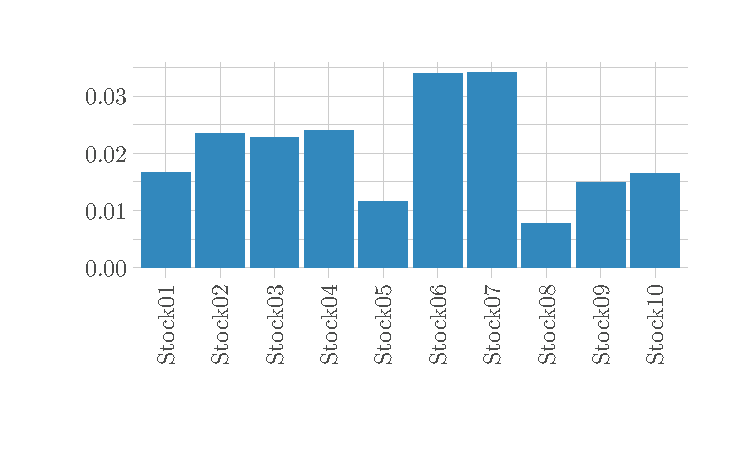
\includegraphics{figures/RiskContribEqual101.pdf}}
		\subfigure[February]{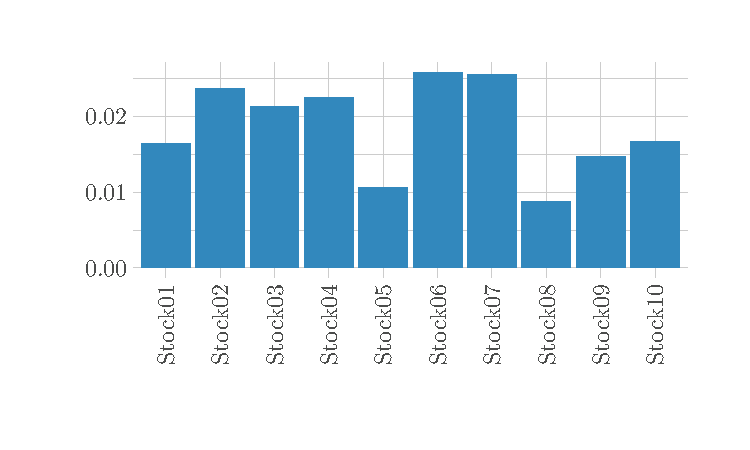
\includegraphics{figures/RiskContribEqual102.pdf}}
		\subfigure[March]{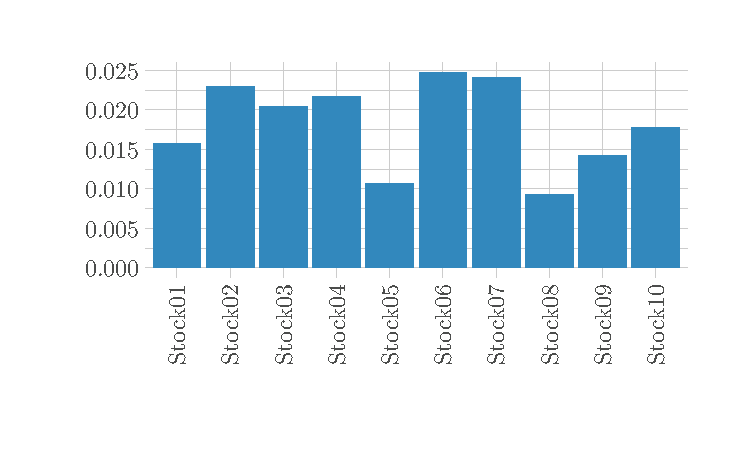
\includegraphics{figures/RiskContribEqual103.pdf}}
		\subfigure[April]{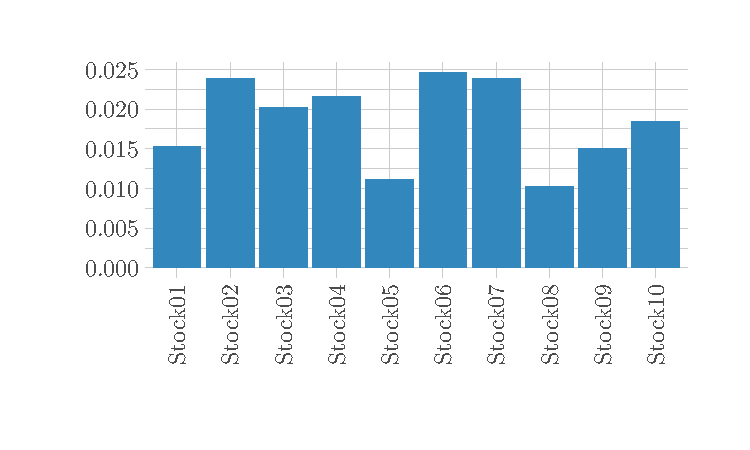
\includegraphics{figures/RiskContribEqual104.pdf}}
		\subfigure[May]{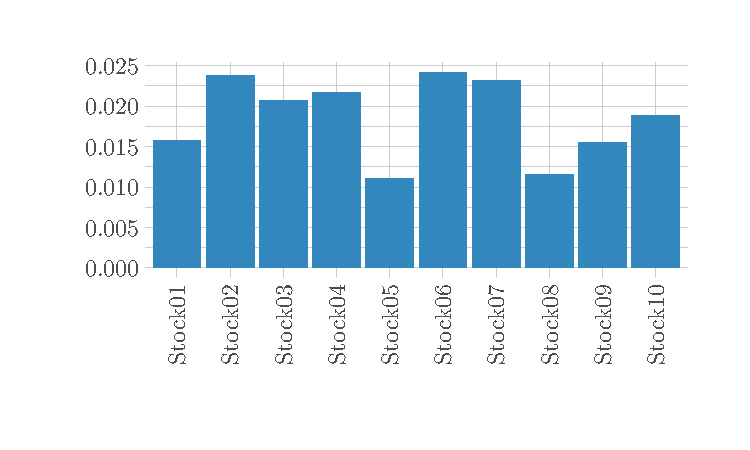
\includegraphics{figures/RiskContribEqual105.pdf}}
		\subfigure[June]{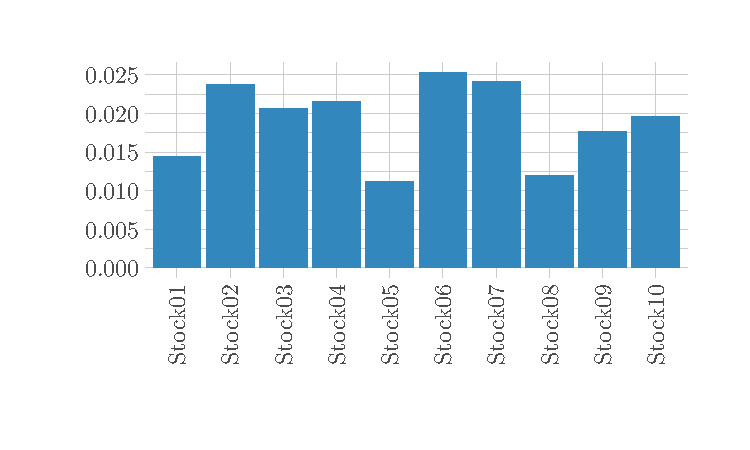
\includegraphics{figures/RiskContribEqual106.pdf}}
	\end{subfigmatrix}
	\caption{Risk Contributions of EWP.}
	\label{fig:condProj1}
	%\end{adjustwidth}
\end{figure}


\begin{figure}[H]
	%\begin{adjustwidth}{2.2cm}{2.2cm}
	\begin{subfigmatrix}{3}
		\subfigure[January]{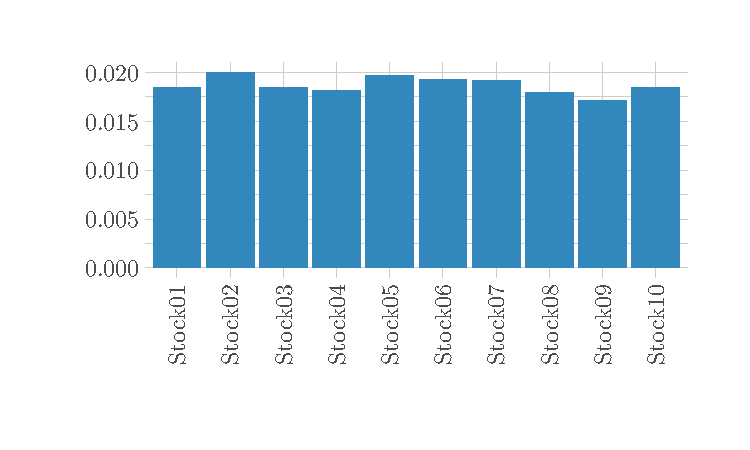
\includegraphics{figures/RiskContrib101.pdf}}
		\subfigure[February]{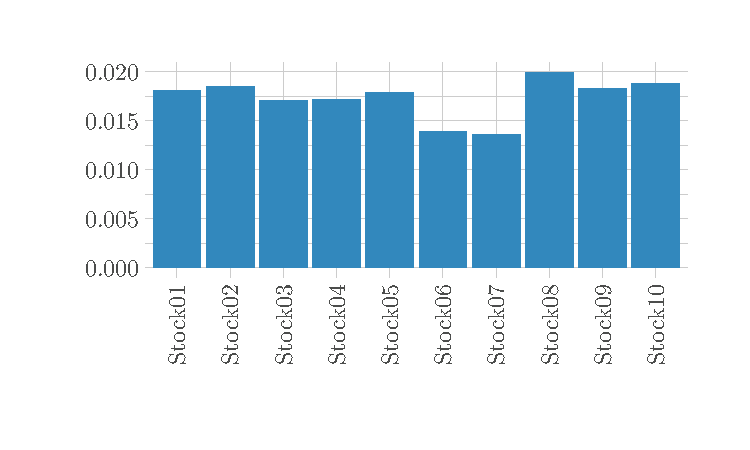
\includegraphics{figures/RiskContrib102.pdf}}
		\subfigure[March]{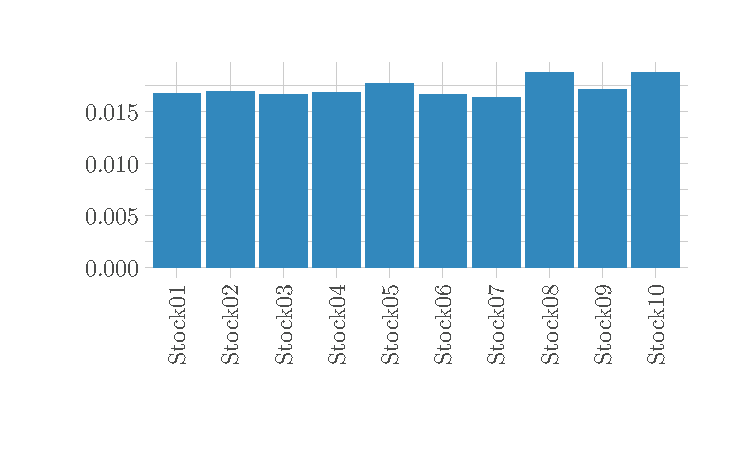
\includegraphics{figures/RiskContrib103.pdf}}
		\subfigure[April]{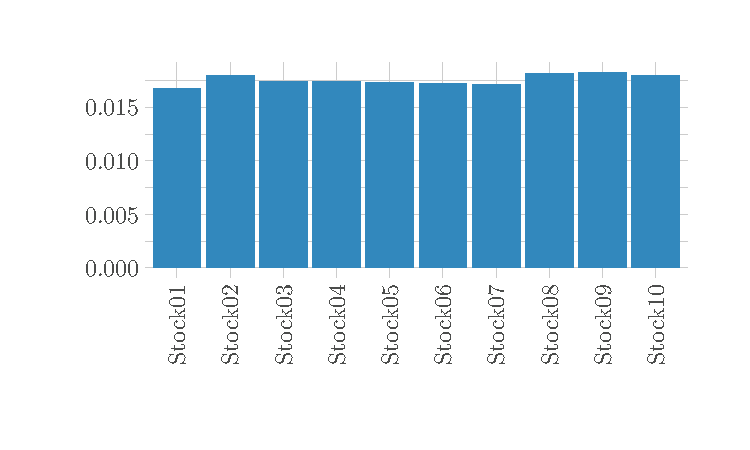
\includegraphics{figures/RiskContrib104.pdf}}
		\subfigure[May]{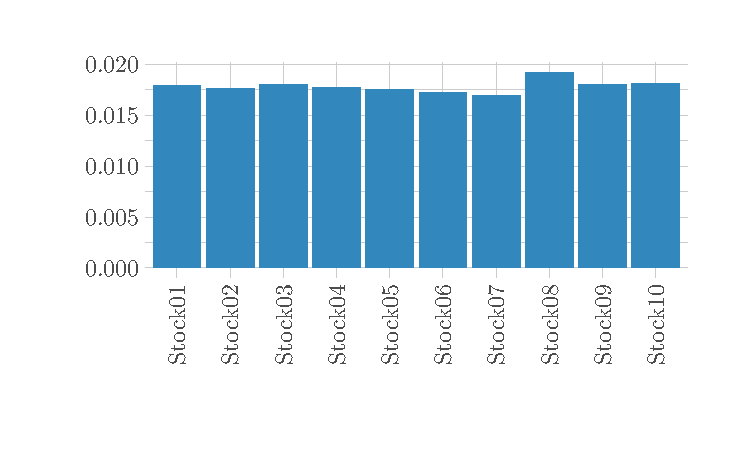
\includegraphics{figures/RiskContrib105.pdf}}
		\subfigure[June]{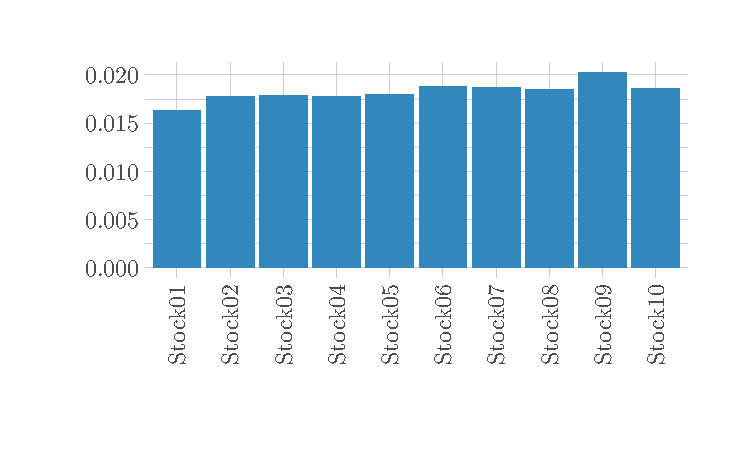
\includegraphics{figures/RiskContrib106.pdf}}
	\end{subfigmatrix}
	\caption{Risk Contributions of RPP.}
	\label{fig:condProj1}
	%\end{adjustwidth}
\end{figure}

\begin{figure}[H]
	\centering
	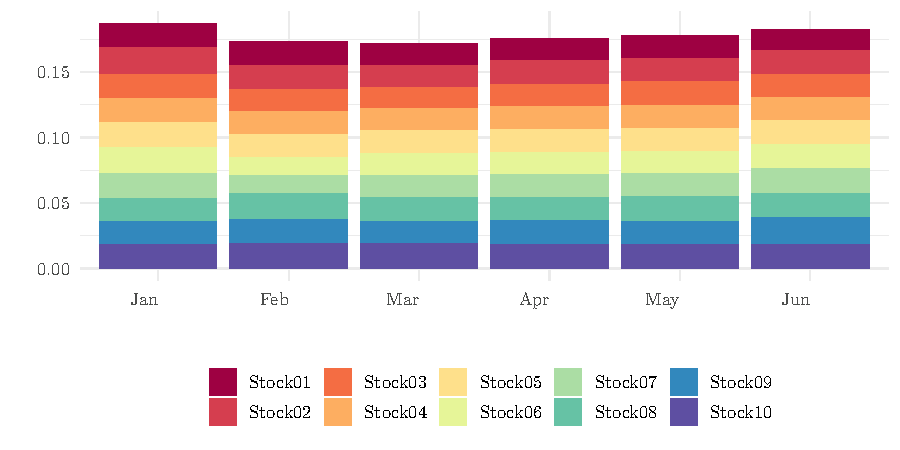
\includegraphics{figures/totalRisk.pdf}
	\caption{Total Risk of RPP.}
	\label{fig:martinezProj}
\end{figure}

\begin{figure}[H]
	\centering
	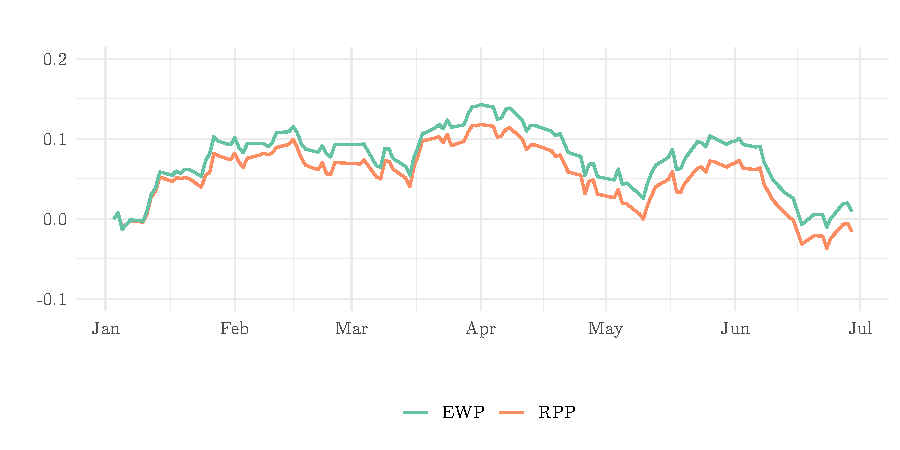
\includegraphics{figures/retornoRPP.pdf}
	\caption{Accumulated Return of EWP and RPP.}
	\label{fig:martinezProj}
\end{figure}

% Let $f(x;b)$ be the function defined by:
% \[
% f(x;b) = \sum_{i=1}^n \big(\mathcal{RC}_i(x) -b_i\mathcal{R}(x)\Big)^2
% \] and the following optimization problem
% \begin{eqnarray}\label{eq:MinProb}
% \min_{x\geq \textbf{0}}\, \{f(x;b)\}; \\
% 	\mbox{s.t. }\left\{
% 	\begin{aligned}\nonumber
% b_i \geq 0, \\
% x_i \geq 0, \\
% {\bf 1}^\top b =1, \\
% {\bf 1}^\top x =1.
% 	\end{aligned}
% 	\right.
% \end{eqnarray}

% If $x^\star$ is the solution to the problem (\ref{eq:MinProb}) and
% $f(x^\star;b)=0$, so $x^\star$ is also system solution
% (\ref{eq:SisNLin}). 


% Roncalli (2013) shows that under the hypothesis that $b_i>0$ the RB portfolio is the solution of the following optimization problem:
% \begin{eqnarray}\label{eq:MinProb}
% \min_{x\geq \textbf{0}}\, \{\mathcal{R}(x)\}; \\
% 	\mbox{s.t. }\left\{
% 	\begin{aligned}\nonumber
% \sum_{i=1}^n b_i \ln(x_i) \geq c, \\
% x_i \geq 0, \\
% {\bf 1}^\top x =1.
% 	\end{aligned}
% 	\right.
% \end{eqnarray}


% In the Gaussian case, when asset returns have a Normal distribution, we can consider $\mathcal{R}(x)=\sigma^2(x)$ and the system (\ref{eq:SisNLin}) reduces to
% \begin{eqnarray}\label{eq:SisGauss}
% x_i (\Sigma x )_i = b_i x^\top \Sigma x,\\
% 	\mbox{s.t. }\left\{
% 	\begin{aligned}\nonumber
% b_i \geq 0, \\
% x_i \geq 0, \\
% {\bf 1}^\top b =1, \\
% {\bf 1}^\top x =1.
% 	\end{aligned}
% 	\right.
% \end{eqnarray}
% for $i=1,2,\dots,n$.


% Setting $w=x/\sqrt{x^\top \Sigma x}$, the equation $x_i (\Sigma x )_i = b_i x^\top \Sigma x$ is equivalent to $w_i(\Sigma w)_i =b_i$, or, in vector form
% \[
% \Sigma w = b^\top/w.
% \]

% Observe that the convex function
% \[
% f(w)= \frac{1}{2}w^\top \Sigma w - b^\top log(w)
% \]
% has a gradient equal to
% \[
% \nabla f(w) = \Sigma w - b^\top/w
% \]
% and the system (\ref{eq:SisGauss}) can be reformulated by the following optimization problem
% \begin{eqnarray}\label{eq:GaussProb}
% \min_{x\geq {\bf 0}}\,\Big\{\frac{1}{2}w^\top \Sigma w - b^\top \log(w)\Big\};  \\
% 	\mbox{s.t. }\left\{
% 	\begin{aligned}\nonumber
% 		\mathbf{1}^\top x=1 & \\
% 		\mathbf{0}\leq x \leq \mathbf{1}
% 	\end{aligned}
% 	\right.
% \end{eqnarray}


% whose optimality condition is $\nabla f(w) = 0$ or $\Sigma w = b/w$ which is precisely the solution of the system (\ref{eq:SisGauss}).



